% ============================================================= %
%  Template LaTeX pour Quarto — Mémoire CNAM style
% ============================================================= 
\documentclass{article}

\usepackage{color}
\usepackage{fancyvrb}
\newcommand{\VerbBar}{|}
\newcommand{\VERB}{\Verb[commandchars=\\\{\}]}
\DefineVerbatimEnvironment{Highlighting}{Verbatim}{commandchars=\\\{\}}
% Add ',fontsize=\small' for more characters per line
\usepackage{framed}
\definecolor{shadecolor}{RGB}{241,243,245}
\newenvironment{Shaded}{\begin{snugshade}}{\end{snugshade}}
\newcommand{\AlertTok}[1]{\textcolor[rgb]{0.68,0.00,0.00}{#1}}
\newcommand{\AnnotationTok}[1]{\textcolor[rgb]{0.37,0.37,0.37}{#1}}
\newcommand{\AttributeTok}[1]{\textcolor[rgb]{0.40,0.45,0.13}{#1}}
\newcommand{\BaseNTok}[1]{\textcolor[rgb]{0.68,0.00,0.00}{#1}}
\newcommand{\BuiltInTok}[1]{\textcolor[rgb]{0.00,0.23,0.31}{#1}}
\newcommand{\CharTok}[1]{\textcolor[rgb]{0.13,0.47,0.30}{#1}}
\newcommand{\CommentTok}[1]{\textcolor[rgb]{0.37,0.37,0.37}{#1}}
\newcommand{\CommentVarTok}[1]{\textcolor[rgb]{0.37,0.37,0.37}{\textit{#1}}}
\newcommand{\ConstantTok}[1]{\textcolor[rgb]{0.56,0.35,0.01}{#1}}
\newcommand{\ControlFlowTok}[1]{\textcolor[rgb]{0.00,0.23,0.31}{\textbf{#1}}}
\newcommand{\DataTypeTok}[1]{\textcolor[rgb]{0.68,0.00,0.00}{#1}}
\newcommand{\DecValTok}[1]{\textcolor[rgb]{0.68,0.00,0.00}{#1}}
\newcommand{\DocumentationTok}[1]{\textcolor[rgb]{0.37,0.37,0.37}{\textit{#1}}}
\newcommand{\ErrorTok}[1]{\textcolor[rgb]{0.68,0.00,0.00}{#1}}
\newcommand{\ExtensionTok}[1]{\textcolor[rgb]{0.00,0.23,0.31}{#1}}
\newcommand{\FloatTok}[1]{\textcolor[rgb]{0.68,0.00,0.00}{#1}}
\newcommand{\FunctionTok}[1]{\textcolor[rgb]{0.28,0.35,0.67}{#1}}
\newcommand{\ImportTok}[1]{\textcolor[rgb]{0.00,0.46,0.62}{#1}}
\newcommand{\InformationTok}[1]{\textcolor[rgb]{0.37,0.37,0.37}{#1}}
\newcommand{\KeywordTok}[1]{\textcolor[rgb]{0.00,0.23,0.31}{\textbf{#1}}}
\newcommand{\NormalTok}[1]{\textcolor[rgb]{0.00,0.23,0.31}{#1}}
\newcommand{\OperatorTok}[1]{\textcolor[rgb]{0.37,0.37,0.37}{#1}}
\newcommand{\OtherTok}[1]{\textcolor[rgb]{0.00,0.23,0.31}{#1}}
\newcommand{\PreprocessorTok}[1]{\textcolor[rgb]{0.68,0.00,0.00}{#1}}
\newcommand{\RegionMarkerTok}[1]{\textcolor[rgb]{0.00,0.23,0.31}{#1}}
\newcommand{\SpecialCharTok}[1]{\textcolor[rgb]{0.37,0.37,0.37}{#1}}
\newcommand{\SpecialStringTok}[1]{\textcolor[rgb]{0.13,0.47,0.30}{#1}}
\newcommand{\StringTok}[1]{\textcolor[rgb]{0.13,0.47,0.30}{#1}}
\newcommand{\VariableTok}[1]{\textcolor[rgb]{0.07,0.07,0.07}{#1}}
\newcommand{\VerbatimStringTok}[1]{\textcolor[rgb]{0.13,0.47,0.30}{#1}}
\newcommand{\WarningTok}[1]{\textcolor[rgb]{0.37,0.37,0.37}{\textit{#1}}}

% ── Packages essentiels ─────────────────────────────────────── 
\usepackage{geometry}
\geometry{a4paper, top=2.5cm, bottom=2.5cm, left=3cm, right=3cm}

\usepackage{microtype}
\usepackage{lmodern}

% ── Couleurs ───────────────────────────────────────────────── 
\usepackage{xcolor}
\usepackage{colortbl}
\definecolor{cnamred}{RGB}{210, 35, 42}
\definecolor{cnamgray}{RGB}{90, 90, 90}
\definecolor{sectionblue}{RGB}{31, 73, 125}
\definecolor{lightgray}{RGB}{245, 245, 245}
\definecolor{rulegray}{RGB}{180, 180, 180}
\definecolor{shadecolor}{RGB}{248, 248, 248}

% ── Graphiques & mise en page ──────────────────────────────── 
\usepackage{graphicx}

% ── Fix pour les images Quarto (pandocbounded) ─────────────── 
\makeatletter
\def\maxwidth{\ifdim\Gin@nat@width>\linewidth\linewidth\else\Gin@nat@width\fi}
\def\maxheight{\ifdim\Gin@nat@height>\textheight\textheight\else\Gin@nat@height\fi}

\newsavebox\pandoc@box
\newcommand*\pandocbounded[1]{%
  \sbox\pandoc@box{#1}%
  \Gscale@div\@tempa{\textheight}{\dimexpr\ht\pandoc@box+\dp\pandoc@box\relax}%
  \Gscale@div\@tempb{\linewidth}{\wd\pandoc@box}%
  \ifdim\@tempb\p@<\@tempa\p@\let\@tempa\@tempb\fi%
  \ifdim\@tempa\p@<\p@\scalebox{\@tempa}{\usebox\pandoc@box}%
  \else\usebox{\pandoc@box}%
  \fi%
}
\makeatother

\usepackage{tikz}
\usepackage{calc}
\usepackage{tabularx}
\usepackage{booktabs}
\usepackage{array}
\usepackage{multirow}
\usepackage{ragged2e}

% ── Typographie des titres ─────────────────────────────────── 
\usepackage{titlesec}

\titleformat{\section}
  {\color{sectionblue}\large\bfseries}
  {\thesection.}{0.6em}{}
  [{\color{rulegray}\vspace{2pt}{\titlerule[0.4pt]}\vspace{4pt}}]

\titleformat{\subsection}
  {\color{sectionblue}\normalsize\bfseries}
  {\thesubsection}{0.6em}{}

\titleformat{\subsubsection}
  {\color{cnamgray}\normalsize\itshape\bfseries}
  {\thesubsubsection}{0.6em}{}

\titlespacing*{\section}{0pt}{18pt}{8pt}
\titlespacing*{\subsection}{0pt}{14pt}{5pt}
\titlespacing*{\subsubsection}{0pt}{10pt}{4pt}

% ── Table des matières ─────────────────────────────────────── 
\usepackage{tocloft}
\renewcommand{\cftsecfont}{\bfseries\color{sectionblue}}
\renewcommand{\cftsecpagefont}{\bfseries\color{sectionblue}}
\renewcommand{\cftsubsecfont}{\color{cnamgray}}
\renewcommand{\cftsubsecpagefont}{\color{cnamgray}}
\renewcommand{\cftsecleader}{\cftdotfill{\cftdotsep}}
\setlength{\cftbeforesecskip}{4pt}

% ── Hyperliens ─────────────────────────────────────────────── 
\usepackage{hyperref}
\hypersetup{
  colorlinks=true,
  linkcolor=sectionblue,
  urlcolor=cnamred,
  citecolor=cnamgray,
  pdfborder={0 0 0}
}

% ── En-têtes et pieds de page ──────────────────────────────── 
\usepackage{fancyhdr}
\pagestyle{fancy}
\fancyhf{}
\fancyhead[L]{\small\color{cnamgray}\textit{Cluster analysis}}
\fancyhead[R]{\small\color{cnamgray}Arsène MBABEH - Raphaël PÉNÉ - Oscar JOSEPH--GENESLAY}
\fancyfoot[C]{\small\color{cnamgray}\thepage}
\renewcommand{\headrulewidth}{0.4pt}
\renewcommand{\footrulewidth}{0pt}

% ── Mathématiques ──────────────────────────────────────────── 
\usepackage{amsmath, amssymb, amsthm}

% ── Bibliographie ──────────────────────────────────────────── 

\usepackage[backend=biber, style=apa]{biblatex}
\addbibresource{references.bib}

% ── Utilitaires Pandoc / Quarto ────────────────────────────── 
\usepackage{longtable}
\usepackage{float}
\usepackage{caption}
\captionsetup{font=small, labelfont={bf,color=sectionblue}, textfont=it}
\usepackage{subcaption}
\usepackage{framed}
\usepackage{wrapfig}
\usepackage{pdflscape}
\usepackage{threeparttable}
\usepackage{threeparttablex}
\usepackage[normalem]{ulem}
\usepackage{makecell}

% ── Fix bug longtable : Pandoc génère \begin{longtable}[]{} ────
%    L'argument optionnel vide [] est interprété comme le compteur
%    "none" qui n'existe pas → on le crée silencieusement.
\makeatletter
\@ifundefined{c@none}{\newcounter{none}}{}
\makeatother

\providecommand{\tightlist}{%
  \setlength{\itemsep}{2pt}\setlength{\parskip}{0pt}}

% ── Interligne & paragraphes ───────────────────────────────── 
\usepackage{setspace}
\setstretch{1.15}
\setlength{\parskip}{6pt}
\setlength{\parindent}{0pt}


% ============================================================= %
%  DOCUMENT
% ============================================================= 
\begin{document}

% ── PAGE DE GARDE ──────────────────────────────────────────── 
\begin{titlepage}
\thispagestyle{empty}

\begin{tikzpicture}[remember picture, overlay]
  \node[anchor=north east, xshift=-1.5cm, yshift=-1.2cm]
    at (current page.north east) {%
      
\includegraphics[width=4cm, keepaspectratio]{logo_cnam.jpg}
    };
\end{tikzpicture}

\vspace*{2cm}

\begin{center}
  {\large\bfseries{Le Conservatoire National des Arts et M\'{e}tiers}}\\[0.4cm]
  \textcolor{rulegray}{\rule{10cm}{0.4pt}}\\[0.6cm]
  {\normalsize Rapport sur la reproductibilité d'un article scientifique sur les archétypes}\\[0.4cm]
  {\normalsize\bfseries Fouille de donn\'{e}es}\\[0.5cm]
  {\small \textit{30 mai 2026} par}\\[0.5cm]
  {\normalsize\bfseries Arsène MBABEH - Raphaël PÉNÉ - Oscar JOSEPH--GENESLAY}\\[0.4cm]
  {\normalsize Promotion (2025-2026)}\\[0.5cm]
  \textcolor{rulegray}{\rule{10cm}{0.4pt}}\\[1.2cm]
  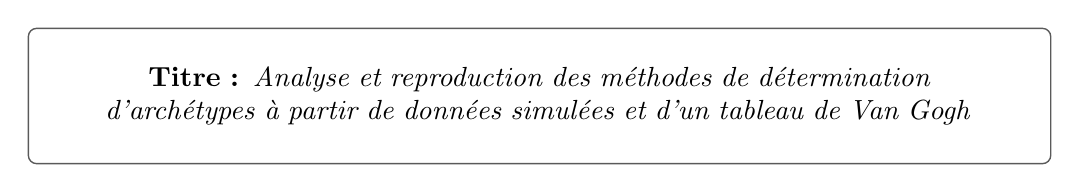
\begin{tikzpicture}
    \node[
      draw=cnamgray,
      line width=0.5pt,
      rounded corners=3pt,
      inner sep=14pt,
      text width=12cm,
      align=center,
      fill=white
    ]{%
      \textbf{Titre :} \textit{Analyse et reproduction des m\'{e}thodes de d\'{e}termination d'arch\'{e}types
      \`{a} partir de donn\'{e}es simul\'{e}es et d'un tableau de Van Gogh}%
    };
  \end{tikzpicture}
\end{center}

\vfill

\begin{center}
  \textcolor{rulegray}{\rule{10cm}{0.4pt}}\\[0.4cm]
  {\small\color{cnamgray} Ann\'{e}e universitaire 2025-2026}
\end{center}

\end{titlepage}

% ── PAGE TABLE DES MATIÈRES ────────────────────────────────── 
\newpage
\thispagestyle{empty}
\renewcommand{\contentsname}{\color{sectionblue}Table des mati\`{e}res}
{
  \hypersetup{linkcolor=sectionblue}
  \tableofcontents
}
\newpage

% ── CORPS DU DOCUMENT ──────────────────────────────────────── 
\setcounter{page}{1}
\pagestyle{fancy}

\section{Les archétypes}\label{les-archuxe9types}

L'article de \textcite{archetypes} présente le package R
\textbf{\texttt{archetypes}}. Un archétype, est d'après le Larousse un
\emph{``Modèle original ou idéal sur lequel est fait un ouvrage, une
œuvre''}. Le travail ici a pour objectif de trouver des points, appelés
archétypes, dans un ensemble d'observations multivariées, qui permettent
à toutes les observations d'être correctement représentées par une
combianaison convexe des archétypes.

\subsection{Cas théorique : le dataset
toy}\label{cas-thuxe9orique-le-dataset-toy}

Chargement des librairies R utilisées dans le projet :

\begin{Shaded}
\begin{Highlighting}[]
\FunctionTok{library}\NormalTok{(archetypes)}
\FunctionTok{library}\NormalTok{(ggplot2)}
\FunctionTok{library}\NormalTok{(imager)}
\FunctionTok{library}\NormalTok{(tidyverse)}
\FunctionTok{library}\NormalTok{(plotly)}
\FunctionTok{library}\NormalTok{(sf)}
\FunctionTok{library}\NormalTok{(scatterplot3d)}
\end{Highlighting}
\end{Shaded}

L'article utilise un jeu de données appelé \textbf{\texttt{toy}} pour
présenter un exemple théorique de la détermination des archétypes. Les
observations de \textbf{\texttt{toy}} sont définies par 2 coordonnées :
x et y.

\begin{Shaded}
\begin{Highlighting}[]
\FunctionTok{data}\NormalTok{(}\StringTok{"toy"}\NormalTok{)}
\end{Highlighting}
\end{Shaded}

\begin{Shaded}
\begin{Highlighting}[]
\FunctionTok{ggplot}\NormalTok{(toy,}\FunctionTok{aes}\NormalTok{(x,y))}\SpecialCharTok{+}
  \FunctionTok{geom\_point}\NormalTok{()}\SpecialCharTok{+}
  \FunctionTok{ggtitle}\NormalTok{(}\StringTok{"Représentation des observations du dataset }\SpecialCharTok{\textbackslash{}"}\StringTok{toy}\SpecialCharTok{\textbackslash{}"}\StringTok{"}\NormalTok{)}\SpecialCharTok{+}
  \FunctionTok{theme\_minimal}\NormalTok{()}
\end{Highlighting}
\end{Shaded}

\pandocbounded{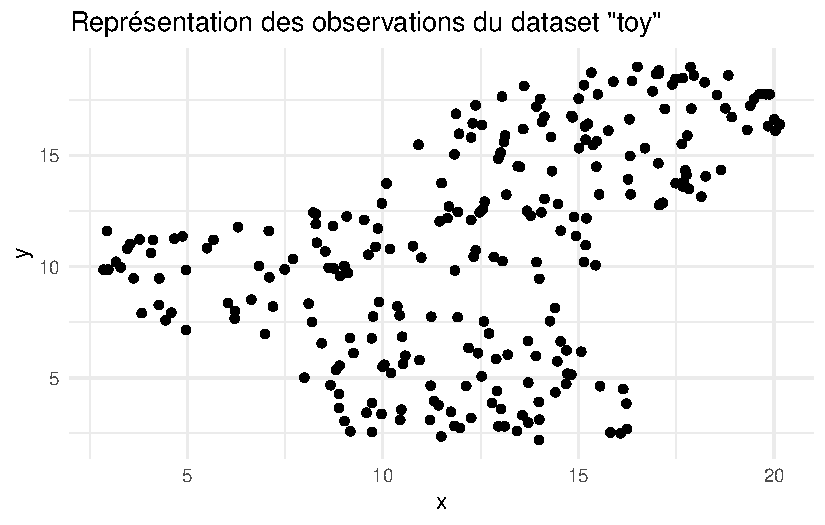
\includegraphics[keepaspectratio]{archetypes_files/figure-pdf/unnamed-chunk-3-1.pdf}}

Les archétypes doivent être placés dans l'enveloppe convexe de la
distribution des données. En effet, on souhaite que les archétypes
soient une combinaison pondérée des individus. La somme des pondérations
doivent être égales à 1. On va essayer de trouver le nombre d'archétypes
optimal pour minimiser la distance entre les individus et les
archétypes.

Résultat de théorème : à partir de 2 archétypes, les archétypes doivent
être sur la bordure de l'enveloppe convexe. Dans l'algorithme, les
archétypes sont placés aléatoirement dans l'enveloppe et les itérations
suivantes déplacent les archétypes vers les extrémités afin de minimiser
les distances. L'algorithme ne connait pas à priori la forme de la
distribution des individus. Attention, ici, comme avec les k-means, les
archétypes trouvés peuvent être un sous-optimum.

On relie les archétypes entre eux par des segments. Les observations
sont projetés sur les segments tracés entre les archétypes. Les points à
l'intérieur de l'enveloppe convexe sont une combinaison des 3
archétypes. Ceux à l'extérieur doivent être projeté. A la fin de la
simulation, le ``bruit'' sont les individus qui ne sont pas dans
l'enveloppe. Pour avoir un bruit égale à 0, il faudrait avoir le même
nombre d'archétypes que le nombre de points sur l'enveloppe convexe.

\begin{Shaded}
\begin{Highlighting}[]
\CommentTok{\# on utilise la même seed que dans l\textquotesingle{}article}
\FunctionTok{set.seed}\NormalTok{(}\DecValTok{1986}\NormalTok{)}

\CommentTok{\# On utilise la fonction archetypes sur le dataset toy, on spécifie le nombre }
\CommentTok{\#d\textquotesingle{}archetypes voulu à 3}
\NormalTok{a }\OtherTok{\textless{}{-}} \FunctionTok{archetypes}\NormalTok{(toy, }\DecValTok{3}\NormalTok{,}\AttributeTok{verbose =} \ConstantTok{TRUE}\NormalTok{)}
\end{Highlighting}
\end{Shaded}

\begin{verbatim}
1: rss = 0.04406432, improvement = 0.07474196
2: rss = 0.04169600, improvement = 0.00236832
3: rss = 0.03907572, improvement = 0.00262028
4: rss = 0.03709453, improvement = 0.00198119
5: rss = 0.03512387, improvement = 0.00197065
6: rss = 0.03393902, improvement = 0.00118485
7: rss = 0.03175524, improvement = 0.00218379
8: rss = 0.02731173, improvement = 0.00444351
9: rss = 0.02055071, improvement = 0.00676101
10: rss = 0.01403723, improvement = 0.00651348
11: rss = 0.01130886, improvement = 0.00272837
12: rss = 0.00977788, improvement = 0.00153098
13: rss = 0.00869493, improvement = 0.00108294
14: rss = 0.00808497, improvement = 0.00060997
15: rss = 0.00774999, improvement = 0.00033498
16: rss = 0.00756613, improvement = 0.00018386
17: rss = 0.00745491, improvement = 0.00011123
18: rss = 0.00738143, improvement = 0.00007348
19: rss = 0.00733080, improvement = 0.00005063
20: rss = 0.00729353, improvement = 0.00003727
21: rss = 0.00728053, improvement = 0.00001300
22: rss = 0.00727438, improvement = 0.00000615
23: rss = 0.00727114, improvement = 0.00000324
24: rss = 0.00726871, improvement = 0.00000243
25: rss = 0.00726710, improvement = 0.00000160
26: rss = 0.00726644, improvement = 0.00000066
27: rss = 0.00726864, improvement = -0.00000220
\end{verbatim}

\begin{Shaded}
\begin{Highlighting}[]
\NormalTok{a}
\end{Highlighting}
\end{Shaded}

\begin{verbatim}
Archetypes object

archetypes(data = toy, k = 3, verbose = TRUE) 

Convergence after 27 iterations
with RSS = 0.007268644.
\end{verbatim}

Chaque itération de la fonction a pour objectif de minimiser le RSS.
Lorsque l'itération suivante fait passer le RSS en négatif, l'algorithme
se stoppe et les coordonnées des archétypes sont trouvées.

\begin{Shaded}
\begin{Highlighting}[]
\CommentTok{\#les coordonnées des archétypes}
\NormalTok{a}\SpecialCharTok{$}\NormalTok{archetypes}
\end{Highlighting}
\end{Shaded}

\begin{verbatim}
             x         y
[1,] 18.832121 18.623102
[2,] 14.204922  2.239856
[3,]  2.872474 10.197810
\end{verbatim}

Nous pouvons maintenant les représenter dans le plan avec les autres
observations :

\pandocbounded{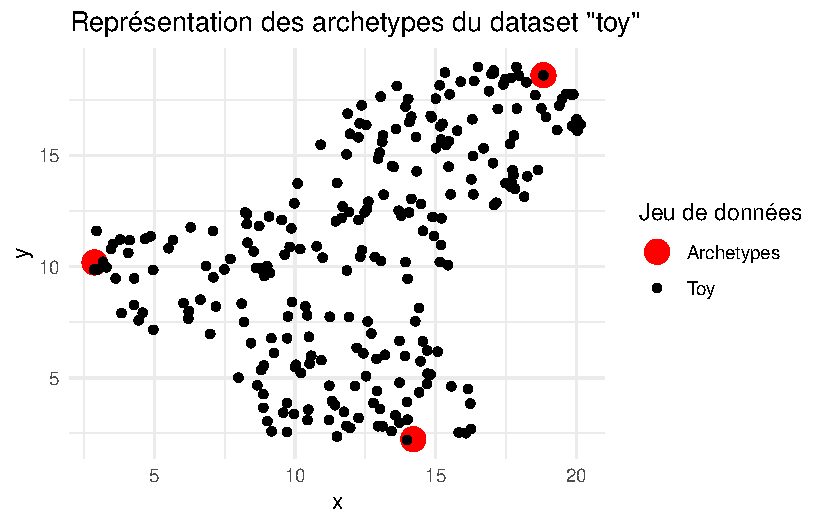
\includegraphics[keepaspectratio]{archetypes_files/figure-pdf/unnamed-chunk-6-1.pdf}}

Maintenant nous pouvons visualiser les observations qui sont dans
l'enveloppe convexe :

\pandocbounded{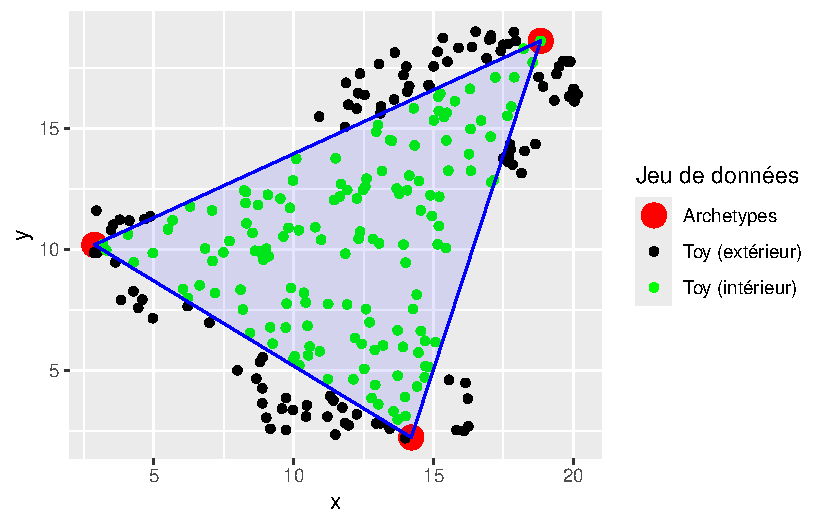
\includegraphics[keepaspectratio]{archetypes_files/figure-pdf/unnamed-chunk-7-1.pdf}}

Nous essayons avec un nombre d'archetypes arbitrairement plus grand.
Avec 4 archetypes :

\begin{Shaded}
\begin{Highlighting}[]
\FunctionTok{set.seed}\NormalTok{(}\DecValTok{1986}\NormalTok{)}
\NormalTok{b }\OtherTok{\textless{}{-}} \FunctionTok{archetypes}\NormalTok{(toy, }\DecValTok{4}\NormalTok{,}\AttributeTok{verbose =} \ConstantTok{TRUE}\NormalTok{)}
\end{Highlighting}
\end{Shaded}

\begin{verbatim}
1: rss = 0.03661230, improvement = 0.05241537
2: rss = 0.03356227, improvement = 0.00305003
3: rss = 0.03009807, improvement = 0.00346420
4: rss = 0.02367849, improvement = 0.00641958
5: rss = 0.01525037, improvement = 0.00842812
6: rss = 0.01065077, improvement = 0.00459960
7: rss = 0.00871585, improvement = 0.00193492
8: rss = 0.00750293, improvement = 0.00121293
9: rss = 0.00665149, improvement = 0.00085144
10: rss = 0.00607836, improvement = 0.00057313
11: rss = 0.00571690, improvement = 0.00036146
12: rss = 0.00550005, improvement = 0.00021685
13: rss = 0.00536954, improvement = 0.00013051
14: rss = 0.00529071, improvement = 0.00007884
15: rss = 0.00525116, improvement = 0.00003955
16: rss = 0.00523391, improvement = 0.00001725
17: rss = 0.00523046, improvement = 0.00000344
18: rss = 0.00523763, improvement = -0.00000717
\end{verbatim}

\begin{Shaded}
\begin{Highlighting}[]
\NormalTok{b}\SpecialCharTok{$}\NormalTok{archetypes}
\end{Highlighting}
\end{Shaded}

\begin{verbatim}
             x         y
[1,] 19.894904 17.767205
[2,]  2.860161  9.941252
[3,] 15.500106 18.779746
[4,] 13.842473  2.218635
\end{verbatim}

\pandocbounded{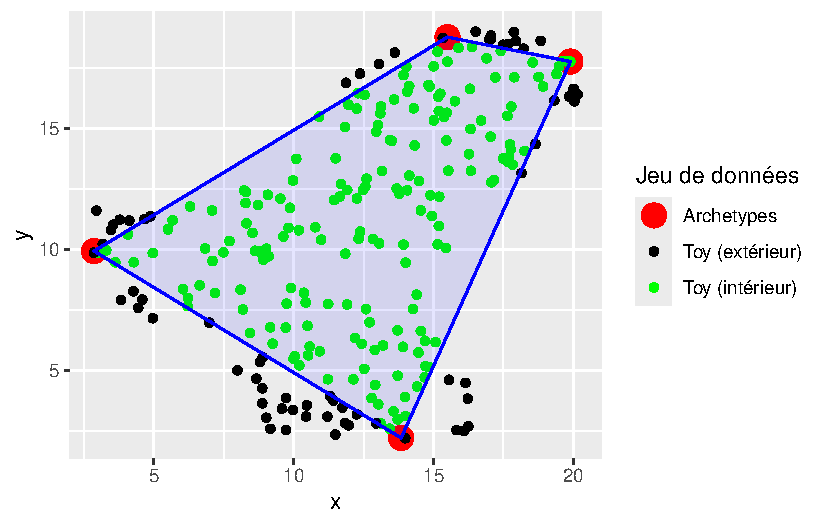
\includegraphics[keepaspectratio]{archetypes_files/figure-pdf/unnamed-chunk-9-1.pdf}}

\subsection{Cas pratique : La Nuit
étoilée}\label{cas-pratique-la-nuit-uxe9toiluxe9e}

Maintenant que nous avons réalisé le projet théorique, nous prenons un
cas pratique avec un tableau. Nous souhaitons trouver les archétypes de
couleur du tableau de Van Gogh \textbf{La nuit étoilée}. Nous
transformons l'image du tableau en data frame. Chaque ligne représente
un pixel de l'image et la valeur de couleur associée. Les copuleurs sont
décrites par le tryptique RGB. Soit rouge R (1), vert G (2), et bleu B
(3). Par pixel nous avons donc 3 lignes pour décrire sa couleur. En
faisant un pivot wider on retrouve une ligne par pixel avec les valeurs
des couleurs RGB dans 3 colonnes distinctes.

\begin{Shaded}
\begin{Highlighting}[]
\NormalTok{img}\OtherTok{\textless{}{-}}\FunctionTok{load.image}\NormalTok{(}\StringTok{\textquotesingle{}nuit\_etoilée.jpeg\textquotesingle{}}\NormalTok{)}
\end{Highlighting}
\end{Shaded}

\begin{Shaded}
\begin{Highlighting}[]
\NormalTok{df }\OtherTok{\textless{}{-}} \FunctionTok{as.data.frame}\NormalTok{(img)}

\NormalTok{df\_rgb }\OtherTok{\textless{}{-}}\NormalTok{ df }\SpecialCharTok{|\textgreater{}} \FunctionTok{pivot\_wider}\NormalTok{(}\AttributeTok{names\_from=}\NormalTok{cc, }\AttributeTok{values\_from =}\NormalTok{ value)}

\NormalTok{df\_rgb }\OtherTok{\textless{}{-}}\NormalTok{ df\_rgb }\SpecialCharTok{|\textgreater{}} \FunctionTok{rename}\NormalTok{(}\AttributeTok{R=}\StringTok{\textquotesingle{}1\textquotesingle{}}\NormalTok{,}\AttributeTok{G=}\StringTok{\textquotesingle{}2\textquotesingle{}}\NormalTok{,}\AttributeTok{B=}\StringTok{\textquotesingle{}3\textquotesingle{}}\NormalTok{)}
\end{Highlighting}
\end{Shaded}

\begin{Shaded}
\begin{Highlighting}[]
\FunctionTok{names}\NormalTok{(df\_rgb)}
\end{Highlighting}
\end{Shaded}

\begin{verbatim}
[1] "x" "y" "R" "G" "B"
\end{verbatim}

\begin{Shaded}
\begin{Highlighting}[]
\FunctionTok{head}\NormalTok{(df\_rgb,}\DecValTok{10}\NormalTok{)}
\end{Highlighting}
\end{Shaded}

\begin{verbatim}
# A tibble: 10 x 5
       x     y      R      G     B
   <int> <int>  <dbl>  <dbl> <dbl>
 1     1     1 0.357  0.333  0.192
 2     2     1 0.255  0.220  0.192
 3     3     1 0.278  0.247  0.306
 4     4     1 0.141  0.125  0.184
 5     5     1 0.173  0.176  0.192
 6     6     1 0.106  0.125  0.149
 7     7     1 0.102  0.114  0.188
 8     8     1 0.0863 0.0941 0.192
 9     9     1 0.141  0.149  0.247
10    10     1 0.157  0.157  0.267
\end{verbatim}

Représentation en 3D d'un échantillon de 50 000 pixels issus du tableau
projetés sur les colonnes R, G et B.

\pandocbounded{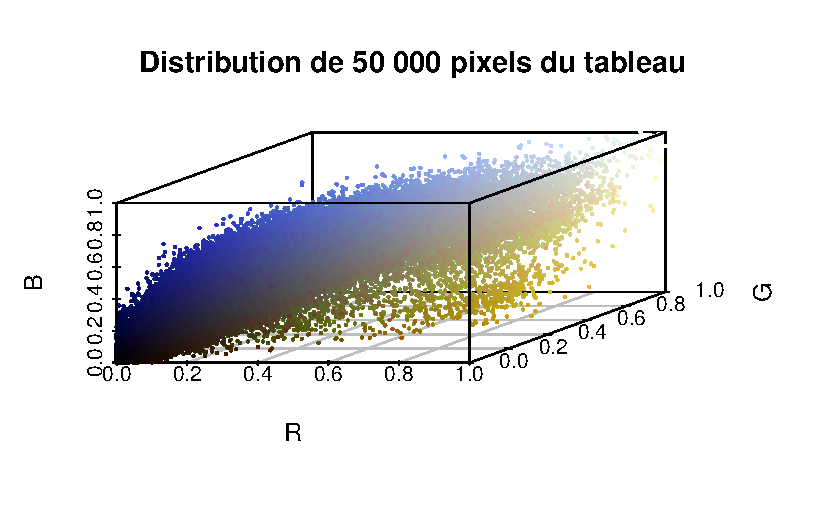
\includegraphics[keepaspectratio]{archetypes_files/figure-pdf/unnamed-chunk-14-1.pdf}}

Nous choisissons arbitrairement de trouver 3 archétypes :

\begin{Shaded}
\begin{Highlighting}[]
\NormalTok{arch}\OtherTok{\textless{}{-}}\FunctionTok{archetypes}\NormalTok{(df\_sample[,}\DecValTok{3}\SpecialCharTok{:}\DecValTok{5}\NormalTok{],}\DecValTok{3}\NormalTok{,}\AttributeTok{verbose =} \ConstantTok{TRUE}\NormalTok{)}
\end{Highlighting}
\end{Shaded}

\begin{verbatim}
1: rss = 0.01609842, improvement = 0.05600228
2: rss = 0.01247558, improvement = 0.00362284
3: rss = 0.01124799, improvement = 0.00122759
4: rss = 0.01062462, improvement = 0.00062338
5: rss = 0.01015625, improvement = 0.00046837
6: rss = 0.00986480, improvement = 0.00029145
7: rss = 0.00967438, improvement = 0.00019042
8: rss = 0.00958970, improvement = 0.00008468
9: rss = 0.00956431, improvement = 0.00002539
10: rss = 0.00956356, improvement = 0.00000075
11: rss = 0.00956558, improvement = -0.00000201
\end{verbatim}

Il faut 14 itérations pour minimiser le RSS et trouver les coordonnées
des 3 archétypes Voici les coordonnées des 3 archétypes :

\begin{Shaded}
\begin{Highlighting}[]
\NormalTok{arch}\SpecialCharTok{$}\NormalTok{archetypes}
\end{Highlighting}
\end{Shaded}

\begin{verbatim}
              R          G          B
[1,] 0.01781294 0.02431116 0.02397419
[2,] 0.85484728 0.85093224 0.63919529
[3,] 0.22352586 0.35686270 0.74119195
\end{verbatim}

Maintenant on peut ajouter ces archétypes à la distribution des 50 000
points :

\pandocbounded{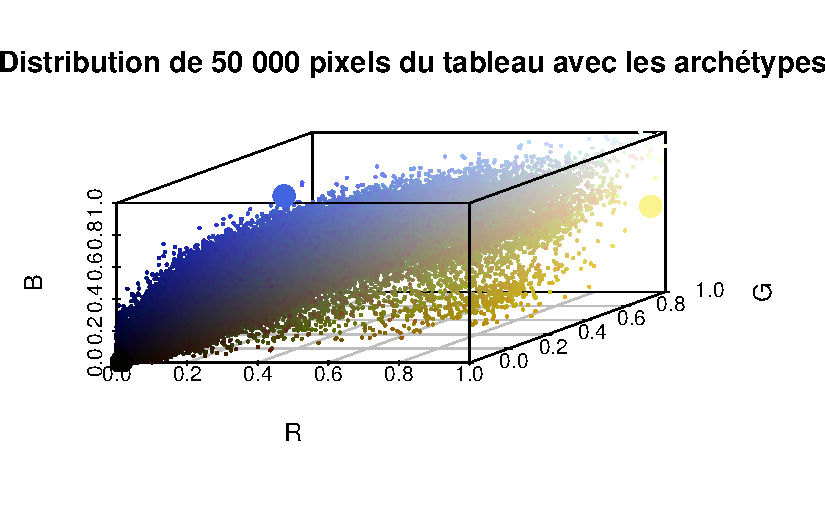
\includegraphics[keepaspectratio]{archetypes_files/figure-pdf/unnamed-chunk-17-1.pdf}}

Nous observons les 3 archetypes : un archétype noir, un archétype bleu
foncé et un archétypes jaune

Nous voulons maintenant déterminer le bon nombre d'archétypes. Nous
utilisons la fonction stepArchetypes en spécifiant la recherche
d'archetypes entre 1 et 5 :

\begin{Shaded}
\begin{Highlighting}[]
\NormalTok{nb\_arche }\OtherTok{\textless{}{-}} \FunctionTok{stepArchetypes}\NormalTok{(df\_sample[}\DecValTok{3}\SpecialCharTok{:}\DecValTok{5}\NormalTok{], }\AttributeTok{k=}\DecValTok{1}\SpecialCharTok{:}\DecValTok{5}\NormalTok{, }\AttributeTok{verbose =} \ConstantTok{FALSE}\NormalTok{, }\AttributeTok{nrep=}\DecValTok{1}\NormalTok{)}
\end{Highlighting}
\end{Shaded}

\begin{verbatim}
Warning in method(..., k = k[i]): k=4: zs > maxKappa
\end{verbatim}

En appliquant le critère du coude nous obtenons le nombre de 3
archétypes, même valeur que celle choisie arbitrairement.

\begin{Shaded}
\begin{Highlighting}[]
\FunctionTok{screeplot}\NormalTok{(nb\_arche)}
\end{Highlighting}
\end{Shaded}

\pandocbounded{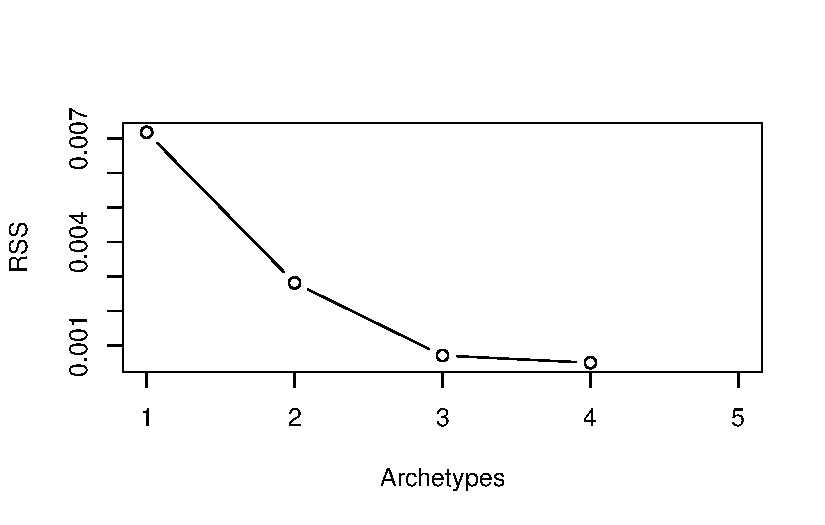
\includegraphics[keepaspectratio]{archetypes_files/figure-pdf/unnamed-chunk-19-1.pdf}}

Nous voulons maintenant revenir à une image avec les 50 000 points que
nous avons choisi aléatoirement. Nous voulons que les 50 000 points
prennent des couleurs liées aux archétypes, c'est à dire projetées sur
le plan formé par les 3 archétypes.

Celà revient à résoudre une équation du style X\_proj=alpha*Z avec Z la
matrice des archétypes et alpha les paramètres qui permettent la
projection.

Transformation des coordonnées des archétypes en matrice :

\begin{Shaded}
\begin{Highlighting}[]
\NormalTok{Z}\OtherTok{=}\FunctionTok{as.matrix}\NormalTok{(arch\_df)}

\NormalTok{Z}
\end{Highlighting}
\end{Shaded}

\begin{verbatim}
              R          G          B
[1,] 0.01781294 0.02431116 0.02397419
[2,] 0.85484728 0.85093224 0.63919529
[3,] 0.22352586 0.35686270 0.74119195
\end{verbatim}

Nous obtenenons les paramètres alphas grâce au paramètre alpha de
l'objet archetypes nommé arch :

\begin{Shaded}
\begin{Highlighting}[]
\NormalTok{alpha}\OtherTok{\textless{}{-}}\NormalTok{arch}\SpecialCharTok{$}\NormalTok{alphas}
\end{Highlighting}
\end{Shaded}

Calcul de la matrice X\_proj :

\begin{Shaded}
\begin{Highlighting}[]
\NormalTok{X\_proj }\OtherTok{\textless{}{-}}\NormalTok{alpha}\SpecialCharTok{\%*\%}\NormalTok{Z}

\NormalTok{X\_proj }\OtherTok{\textless{}{-}} \FunctionTok{as.data.frame}\NormalTok{(X\_proj)}
\end{Highlighting}
\end{Shaded}

Représentation dans l'espace des points projetés sur le plan crée par
les archétypes :

\begin{Shaded}
\begin{Highlighting}[]
\CommentTok{\# Couleurs des points (couleurs réelles depuis df\_sample) et des archétypes}
\NormalTok{colors\_sample }\OtherTok{\textless{}{-}} \FunctionTok{adjustcolor}\NormalTok{(}
  \FunctionTok{rgb}\NormalTok{(df\_sample}\SpecialCharTok{$}\NormalTok{R, df\_sample}\SpecialCharTok{$}\NormalTok{G, df\_sample}\SpecialCharTok{$}\NormalTok{B),}
  \AttributeTok{alpha.f =} \FloatTok{0.5}
\NormalTok{)}
\NormalTok{colors\_arch }\OtherTok{\textless{}{-}} \FunctionTok{rgb}\NormalTok{(arch\_df}\SpecialCharTok{$}\NormalTok{R, arch\_df}\SpecialCharTok{$}\NormalTok{G, arch\_df}\SpecialCharTok{$}\NormalTok{B)}

\CommentTok{\# Graphique de base avec les coordonnées projetées (X\_proj) mais couleurs réelles (df\_sample)}
\NormalTok{s3d }\OtherTok{\textless{}{-}} \FunctionTok{scatterplot3d}\NormalTok{(}
  \AttributeTok{x          =}\NormalTok{ X\_proj}\SpecialCharTok{$}\NormalTok{R,}
  \AttributeTok{y          =}\NormalTok{ X\_proj}\SpecialCharTok{$}\NormalTok{G,}
  \AttributeTok{z          =}\NormalTok{ X\_proj}\SpecialCharTok{$}\NormalTok{B,}
  \AttributeTok{color      =}\NormalTok{ colors\_sample,}
  \AttributeTok{pch        =} \DecValTok{16}\NormalTok{,}
  \AttributeTok{cex.symbol =} \FloatTok{0.3}\NormalTok{,}
  \AttributeTok{xlab       =} \StringTok{"R"}\NormalTok{,}
  \AttributeTok{ylab       =} \StringTok{"G"}\NormalTok{,}
  \AttributeTok{zlab       =} \StringTok{"B"}\NormalTok{,}
  \AttributeTok{xlim       =} \FunctionTok{c}\NormalTok{(}\DecValTok{0}\NormalTok{, }\DecValTok{1}\NormalTok{),}
  \AttributeTok{ylim       =} \FunctionTok{c}\NormalTok{(}\DecValTok{0}\NormalTok{, }\DecValTok{1}\NormalTok{),}
  \AttributeTok{zlim       =} \FunctionTok{c}\NormalTok{(}\DecValTok{0}\NormalTok{, }\DecValTok{1}\NormalTok{),}
  \AttributeTok{main       =} \StringTok{"Distribution de 50 000 pixels du tableau projetés dans }
\StringTok{  le plan formé par les archétypes"}
\NormalTok{)}

\CommentTok{\# Ajout des archétypes}
\NormalTok{s3d}\SpecialCharTok{$}\FunctionTok{points3d}\NormalTok{(}
  \AttributeTok{x   =}\NormalTok{ arch\_df}\SpecialCharTok{$}\NormalTok{R,}
  \AttributeTok{y   =}\NormalTok{ arch\_df}\SpecialCharTok{$}\NormalTok{G,}
  \AttributeTok{z   =}\NormalTok{ arch\_df}\SpecialCharTok{$}\NormalTok{B,}
  \AttributeTok{col =}\NormalTok{ colors\_arch,}
  \AttributeTok{pch =} \DecValTok{16}\NormalTok{,}
  \AttributeTok{cex =} \DecValTok{2}
\NormalTok{)}
\end{Highlighting}
\end{Shaded}

\pandocbounded{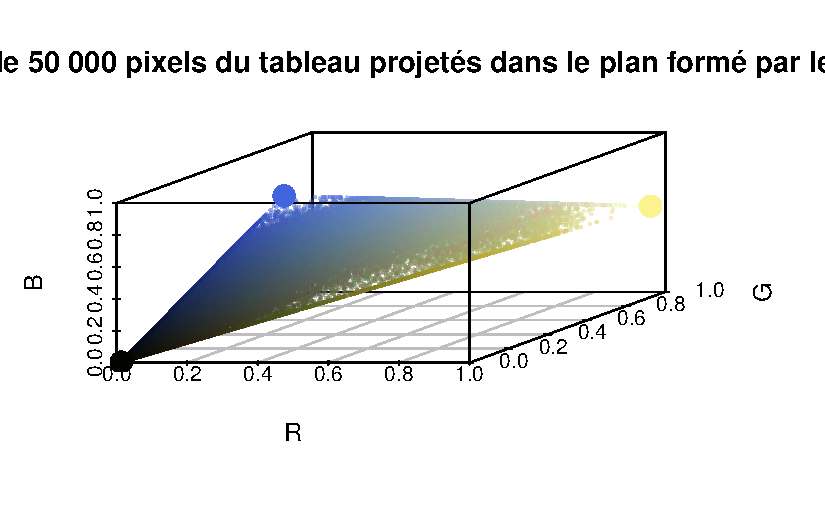
\includegraphics[keepaspectratio]{archetypes_files/figure-pdf/unnamed-chunk-24-1.pdf}}

Nous observons que tous les points sont bien projetés sur le plan crée
par les 3 archétypes ou sur les segments tracés entre les archétypes.

Nous souhaitons maintenant repositionner ces pixels avec leur nouvelle
couleur sur le tableau d'origine :

\begin{Shaded}
\begin{Highlighting}[]
\NormalTok{df\_proj }\OtherTok{\textless{}{-}} \FunctionTok{cbind}\NormalTok{(df\_sample[,}\DecValTok{1}\SpecialCharTok{:}\DecValTok{2}\NormalTok{],X\_proj)}
\end{Highlighting}
\end{Shaded}

\begin{Shaded}
\begin{Highlighting}[]
\NormalTok{image\_proj }\OtherTok{\textless{}{-}}\NormalTok{ df\_proj }\SpecialCharTok{|\textgreater{}} \FunctionTok{pivot\_longer}\NormalTok{( }\AttributeTok{cols =} \FunctionTok{c}\NormalTok{(}\StringTok{"R"}\NormalTok{,}\StringTok{"G"}\NormalTok{,}\StringTok{"B"}\NormalTok{), }\AttributeTok{names\_to =} \StringTok{"canal"}\NormalTok{, }\AttributeTok{values\_to =} \StringTok{"value"}\NormalTok{) }\SpecialCharTok{|\textgreater{}} 

  \FunctionTok{mutate}\NormalTok{(}\AttributeTok{cc =} \FunctionTok{match}\NormalTok{(canal, }\FunctionTok{c}\NormalTok{(}\StringTok{"R"}\NormalTok{,}\StringTok{"G"}\NormalTok{,}\StringTok{"B"}\NormalTok{))) }\SpecialCharTok{|\textgreater{}} 

  \FunctionTok{select}\NormalTok{(x,y,cc,value)}

\NormalTok{image\_proj }\OtherTok{\textless{}{-}} \FunctionTok{as.cimg}\NormalTok{(image\_proj)}
\end{Highlighting}
\end{Shaded}

\begin{verbatim}
Warning in as.cimg.data.frame(image_proj): Guessing image dimensions from
maximum coordinate values
\end{verbatim}

\begin{Shaded}
\begin{Highlighting}[]
\FunctionTok{plot}\NormalTok{(image\_proj)}
\end{Highlighting}
\end{Shaded}

\pandocbounded{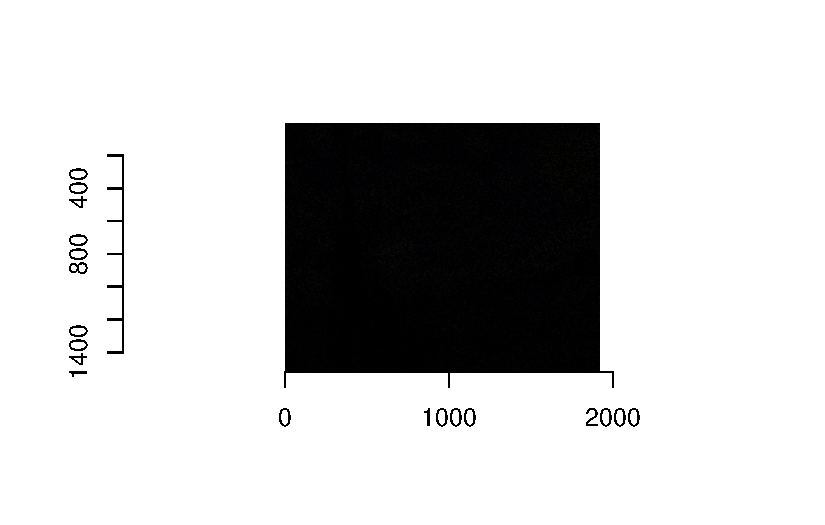
\includegraphics[keepaspectratio]{archetypes_files/figure-pdf/unnamed-chunk-26-1.pdf}}

Les 50 000 points choisis aléatoirements sont difficilement visibles sur
la toile qui en compte en réalité presque 3 millions.

\subsubsection{Trouver les alphas pour l'ensemble des 3 millions de
pixel}\label{trouver-les-alphas-pour-lensemble-des-3-millions-de-pixel}

Nous utilisons la fonction predict. \textbf{Expliquer cette fonction}

\begin{Shaded}
\begin{Highlighting}[]
\NormalTok{alphas}\OtherTok{\textless{}{-}}\FunctionTok{predict}\NormalTok{(arch,df\_rgb[,}\DecValTok{3}\SpecialCharTok{:}\DecValTok{5}\NormalTok{])}
\end{Highlighting}
\end{Shaded}

\begin{Shaded}
\begin{Highlighting}[]
\NormalTok{X\_tilde}\OtherTok{\textless{}{-}}\NormalTok{alphas }\SpecialCharTok{\%*\%}\NormalTok{ Z}

\FunctionTok{colnames}\NormalTok{(X\_tilde) }\OtherTok{\textless{}{-}} \FunctionTok{c}\NormalTok{(}\StringTok{"R"}\NormalTok{, }\StringTok{"G"}\NormalTok{, }\StringTok{"B"}\NormalTok{)}

\NormalTok{X\_tilde}\OtherTok{\textless{}{-}}\FunctionTok{cbind}\NormalTok{(df\_rgb[,}\DecValTok{1}\SpecialCharTok{:}\DecValTok{2}\NormalTok{],X\_tilde)}
\end{Highlighting}
\end{Shaded}

\begin{Shaded}
\begin{Highlighting}[]
\NormalTok{image\_proj }\OtherTok{\textless{}{-}}\NormalTok{ X\_tilde }\SpecialCharTok{|\textgreater{}} \FunctionTok{pivot\_longer}\NormalTok{( }\AttributeTok{cols =} \FunctionTok{c}\NormalTok{(}\StringTok{"R"}\NormalTok{,}\StringTok{"G"}\NormalTok{,}\StringTok{"B"}\NormalTok{), }\AttributeTok{names\_to =} \StringTok{"canal"}\NormalTok{, }\AttributeTok{values\_to =} \StringTok{"value"}\NormalTok{) }\SpecialCharTok{|\textgreater{}}

  \FunctionTok{mutate}\NormalTok{(}\AttributeTok{cc =} \FunctionTok{match}\NormalTok{(canal, }\FunctionTok{c}\NormalTok{(}\StringTok{"R"}\NormalTok{,}\StringTok{"G"}\NormalTok{,}\StringTok{"B"}\NormalTok{))) }\SpecialCharTok{|\textgreater{}}

  \FunctionTok{select}\NormalTok{(x,y,cc,value)}

\NormalTok{image\_proj }\OtherTok{\textless{}{-}} \FunctionTok{as.cimg}\NormalTok{(image\_proj)}
\end{Highlighting}
\end{Shaded}

\begin{verbatim}
Warning in as.cimg.data.frame(image_proj): Guessing image dimensions from
maximum coordinate values
\end{verbatim}

\begin{Shaded}
\begin{Highlighting}[]
\FunctionTok{plot}\NormalTok{(image\_proj)}
\end{Highlighting}
\end{Shaded}

\pandocbounded{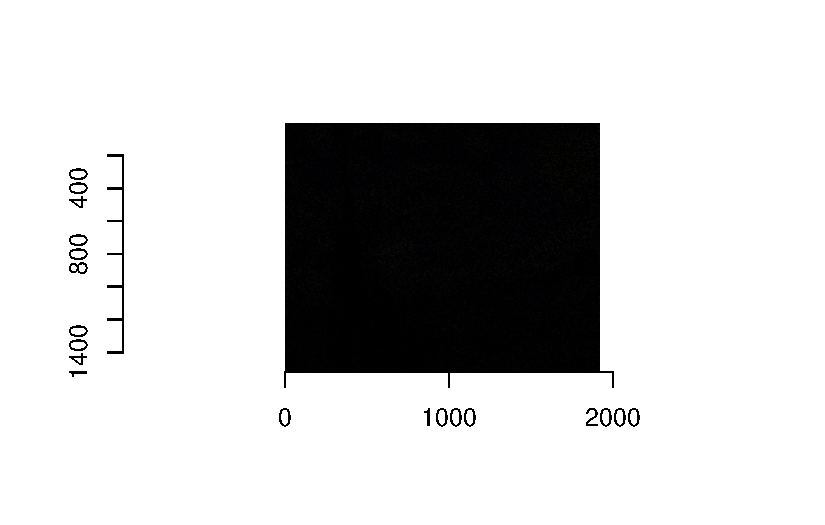
\includegraphics[keepaspectratio]{archetypes_files/figure-pdf/unnamed-chunk-28-1.pdf}}

Nous vérifions que les pixels trouvés font bien partis du plan crée par
les 3 archétypes. Nous prenons un échantillons de 200 000 pixels :

\begin{Shaded}
\begin{Highlighting}[]
\CommentTok{\# Échantillonnage}
\NormalTok{ech }\OtherTok{\textless{}{-}}\NormalTok{ X\_tilde[}\FunctionTok{sample}\NormalTok{(}\DecValTok{1}\SpecialCharTok{:}\DecValTok{2918400}\NormalTok{, }\DecValTok{200000}\NormalTok{), ]}

\CommentTok{\# Couleurs}
\NormalTok{colors\_ech  }\OtherTok{\textless{}{-}} \FunctionTok{adjustcolor}\NormalTok{(}
  \FunctionTok{rgb}\NormalTok{(ech}\SpecialCharTok{$}\NormalTok{R, ech}\SpecialCharTok{$}\NormalTok{G, ech}\SpecialCharTok{$}\NormalTok{B),}
  \AttributeTok{alpha.f =} \FloatTok{0.5}
\NormalTok{)}
\NormalTok{colors\_arch }\OtherTok{\textless{}{-}} \FunctionTok{rgb}\NormalTok{(arch\_df}\SpecialCharTok{$}\NormalTok{R, arch\_df}\SpecialCharTok{$}\NormalTok{G, arch\_df}\SpecialCharTok{$}\NormalTok{B)}

\CommentTok{\# Graphique principal}
\NormalTok{s3d }\OtherTok{\textless{}{-}} \FunctionTok{scatterplot3d}\NormalTok{(}
  \AttributeTok{x          =}\NormalTok{ ech}\SpecialCharTok{$}\NormalTok{R,}
  \AttributeTok{y          =}\NormalTok{ ech}\SpecialCharTok{$}\NormalTok{G,}
  \AttributeTok{z          =}\NormalTok{ ech}\SpecialCharTok{$}\NormalTok{B,}
  \AttributeTok{color      =}\NormalTok{ colors\_ech,}
  \AttributeTok{pch        =} \DecValTok{16}\NormalTok{,}
  \AttributeTok{cex.symbol =} \FloatTok{0.3}\NormalTok{,}
  \AttributeTok{xlab       =} \StringTok{"R"}\NormalTok{,}
  \AttributeTok{ylab       =} \StringTok{"G"}\NormalTok{,}
  \AttributeTok{zlab       =} \StringTok{"B"}\NormalTok{,}
  \AttributeTok{xlim       =} \FunctionTok{c}\NormalTok{(}\DecValTok{0}\NormalTok{, }\DecValTok{1}\NormalTok{),}
  \AttributeTok{ylim       =} \FunctionTok{c}\NormalTok{(}\DecValTok{0}\NormalTok{, }\DecValTok{1}\NormalTok{),}
  \AttributeTok{zlim       =} \FunctionTok{c}\NormalTok{(}\DecValTok{0}\NormalTok{, }\DecValTok{1}\NormalTok{),}
  \AttributeTok{main       =} \StringTok{"Distribution de 200 000 pixels obtenus avec la fonction predict"}
\NormalTok{)}

\CommentTok{\# Ajout des archétypes}
\NormalTok{s3d}\SpecialCharTok{$}\FunctionTok{points3d}\NormalTok{(}
  \AttributeTok{x   =}\NormalTok{ arch\_df}\SpecialCharTok{$}\NormalTok{R,}
  \AttributeTok{y   =}\NormalTok{ arch\_df}\SpecialCharTok{$}\NormalTok{G,}
  \AttributeTok{z   =}\NormalTok{ arch\_df}\SpecialCharTok{$}\NormalTok{B,}
  \AttributeTok{col =}\NormalTok{ colors\_arch,}
  \AttributeTok{pch =} \DecValTok{16}\NormalTok{,}
  \AttributeTok{cex =} \DecValTok{2}
\NormalTok{)}
\end{Highlighting}
\end{Shaded}

\pandocbounded{\includegraphics[keepaspectratio]{archetypes_files/figure-pdf/unnamed-chunk-30-1.pdf}}

\subsubsection{Avec 2 archétypes}\label{avec-2-archuxe9types}

\begin{Shaded}
\begin{Highlighting}[]
\NormalTok{arch}\OtherTok{\textless{}{-}}\FunctionTok{archetypes}\NormalTok{(df\_sample[,}\DecValTok{3}\SpecialCharTok{:}\DecValTok{5}\NormalTok{],}\DecValTok{2}\NormalTok{,}\AttributeTok{verbose =} \ConstantTok{TRUE}\NormalTok{)}
\end{Highlighting}
\end{Shaded}

\begin{verbatim}
1: rss = 0.04244395, improvement = 0.10274193
2: rss = 0.03028907, improvement = 0.01215488
3: rss = 0.02883565, improvement = 0.00145342
4: rss = 0.02854787, improvement = 0.00028779
5: rss = 0.02831588, improvement = 0.00023199
6: rss = 0.02811448, improvement = 0.00020139
7: rss = 0.02796552, improvement = 0.00014896
8: rss = 0.02786832, improvement = 0.00009720
9: rss = 0.02781305, improvement = 0.00005527
10: rss = 0.02778222, improvement = 0.00003082
11: rss = 0.02776492, improvement = 0.00001730
12: rss = 0.02775492, improvement = 0.00001000
13: rss = 0.02774884, improvement = 0.00000608
14: rss = 0.02774715, improvement = 0.00000169
15: rss = 0.02774785, improvement = -0.00000069
\end{verbatim}

\begin{Shaded}
\begin{Highlighting}[]
\NormalTok{alphas}\OtherTok{\textless{}{-}}\FunctionTok{predict}\NormalTok{(arch,df\_rgb[,}\DecValTok{3}\SpecialCharTok{:}\DecValTok{5}\NormalTok{])}
\end{Highlighting}
\end{Shaded}

\begin{Shaded}
\begin{Highlighting}[]
\NormalTok{arch\_df }\OtherTok{\textless{}{-}} \FunctionTok{as.data.frame}\NormalTok{(arch}\SpecialCharTok{$}\NormalTok{archetypes)}

\FunctionTok{colnames}\NormalTok{(arch\_df) }\OtherTok{\textless{}{-}} \FunctionTok{c}\NormalTok{(}\StringTok{"R"}\NormalTok{, }\StringTok{"G"}\NormalTok{, }\StringTok{"B"}\NormalTok{)}
\end{Highlighting}
\end{Shaded}

\begin{Shaded}
\begin{Highlighting}[]
\NormalTok{Z}\OtherTok{=}\FunctionTok{as.matrix}\NormalTok{(arch\_df)}

\NormalTok{Z}
\end{Highlighting}
\end{Shaded}

\begin{verbatim}
                 R          G         B
[1,] -3.660914e-05 0.04072346 0.1508445
[2,]  7.094321e-01 0.78869288 0.8066049
\end{verbatim}

\begin{Shaded}
\begin{Highlighting}[]
\NormalTok{X\_tilde}\OtherTok{\textless{}{-}}\NormalTok{alphas }\SpecialCharTok{\%*\%}\NormalTok{ Z}

\FunctionTok{colnames}\NormalTok{(X\_tilde) }\OtherTok{\textless{}{-}} \FunctionTok{c}\NormalTok{(}\StringTok{"R"}\NormalTok{, }\StringTok{"G"}\NormalTok{, }\StringTok{"B"}\NormalTok{)}

\NormalTok{X\_tilde}\OtherTok{\textless{}{-}}\FunctionTok{cbind}\NormalTok{(df\_rgb[,}\DecValTok{1}\SpecialCharTok{:}\DecValTok{2}\NormalTok{],X\_tilde)}
\end{Highlighting}
\end{Shaded}

\begin{Shaded}
\begin{Highlighting}[]
\NormalTok{image\_proj }\OtherTok{\textless{}{-}}\NormalTok{ X\_tilde }\SpecialCharTok{|\textgreater{}} \FunctionTok{pivot\_longer}\NormalTok{( }\AttributeTok{cols =} \FunctionTok{c}\NormalTok{(}\StringTok{"R"}\NormalTok{,}\StringTok{"G"}\NormalTok{,}\StringTok{"B"}\NormalTok{), }\AttributeTok{names\_to =} \StringTok{"canal"}\NormalTok{, }\AttributeTok{values\_to =} \StringTok{"value"}\NormalTok{) }\SpecialCharTok{|\textgreater{}}

  \FunctionTok{mutate}\NormalTok{(}\AttributeTok{cc =} \FunctionTok{match}\NormalTok{(canal, }\FunctionTok{c}\NormalTok{(}\StringTok{"R"}\NormalTok{,}\StringTok{"G"}\NormalTok{,}\StringTok{"B"}\NormalTok{))) }\SpecialCharTok{|\textgreater{}}

  \FunctionTok{select}\NormalTok{(x,y,cc,value)}

\NormalTok{image\_proj }\OtherTok{\textless{}{-}} \FunctionTok{as.cimg}\NormalTok{(image\_proj)}
\end{Highlighting}
\end{Shaded}

\begin{verbatim}
Warning in as.cimg.data.frame(image_proj): Guessing image dimensions from
maximum coordinate values
\end{verbatim}

\begin{Shaded}
\begin{Highlighting}[]
\FunctionTok{plot}\NormalTok{(image\_proj)}
\end{Highlighting}
\end{Shaded}

\pandocbounded{\includegraphics[keepaspectratio]{archetypes_files/figure-pdf/unnamed-chunk-34-1.pdf}}

\begin{Shaded}
\begin{Highlighting}[]
\NormalTok{ech }\OtherTok{\textless{}{-}}\NormalTok{ X\_tilde[}\FunctionTok{sample}\NormalTok{(}\DecValTok{1}\SpecialCharTok{:}\DecValTok{2918400}\NormalTok{, }\DecValTok{200000}\NormalTok{), ]}

\CommentTok{\# Clamp RGB to [0, 1] to absorb floating{-}point drift}
\NormalTok{ech}\SpecialCharTok{$}\NormalTok{R }\OtherTok{\textless{}{-}} \FunctionTok{pmax}\NormalTok{(}\DecValTok{0}\NormalTok{, }\FunctionTok{pmin}\NormalTok{(}\DecValTok{1}\NormalTok{, ech}\SpecialCharTok{$}\NormalTok{R))}
\NormalTok{ech}\SpecialCharTok{$}\NormalTok{G }\OtherTok{\textless{}{-}} \FunctionTok{pmax}\NormalTok{(}\DecValTok{0}\NormalTok{, }\FunctionTok{pmin}\NormalTok{(}\DecValTok{1}\NormalTok{, ech}\SpecialCharTok{$}\NormalTok{G))}
\NormalTok{ech}\SpecialCharTok{$}\NormalTok{B }\OtherTok{\textless{}{-}} \FunctionTok{pmax}\NormalTok{(}\DecValTok{0}\NormalTok{, }\FunctionTok{pmin}\NormalTok{(}\DecValTok{1}\NormalTok{, ech}\SpecialCharTok{$}\NormalTok{B))}

\NormalTok{arch\_df}\SpecialCharTok{$}\NormalTok{R }\OtherTok{\textless{}{-}} \FunctionTok{pmax}\NormalTok{(}\DecValTok{0}\NormalTok{, }\FunctionTok{pmin}\NormalTok{(}\DecValTok{1}\NormalTok{, arch\_df}\SpecialCharTok{$}\NormalTok{R))}
\NormalTok{arch\_df}\SpecialCharTok{$}\NormalTok{G }\OtherTok{\textless{}{-}} \FunctionTok{pmax}\NormalTok{(}\DecValTok{0}\NormalTok{, }\FunctionTok{pmin}\NormalTok{(}\DecValTok{1}\NormalTok{, arch\_df}\SpecialCharTok{$}\NormalTok{G))}
\NormalTok{arch\_df}\SpecialCharTok{$}\NormalTok{B }\OtherTok{\textless{}{-}} \FunctionTok{pmax}\NormalTok{(}\DecValTok{0}\NormalTok{, }\FunctionTok{pmin}\NormalTok{(}\DecValTok{1}\NormalTok{, arch\_df}\SpecialCharTok{$}\NormalTok{B))}

\CommentTok{\# Couleurs}
\NormalTok{colors\_ech  }\OtherTok{\textless{}{-}} \FunctionTok{adjustcolor}\NormalTok{(}
  \FunctionTok{rgb}\NormalTok{(ech}\SpecialCharTok{$}\NormalTok{R, ech}\SpecialCharTok{$}\NormalTok{G, ech}\SpecialCharTok{$}\NormalTok{B),}
  \AttributeTok{alpha.f =} \FloatTok{0.5}
\NormalTok{)}
\NormalTok{colors\_arch }\OtherTok{\textless{}{-}} \FunctionTok{rgb}\NormalTok{(arch\_df}\SpecialCharTok{$}\NormalTok{R, arch\_df}\SpecialCharTok{$}\NormalTok{G, arch\_df}\SpecialCharTok{$}\NormalTok{B)}

\CommentTok{\# Graphique principal}
\NormalTok{s3d }\OtherTok{\textless{}{-}} \FunctionTok{scatterplot3d}\NormalTok{(}
  \AttributeTok{x          =}\NormalTok{ ech}\SpecialCharTok{$}\NormalTok{R,}
  \AttributeTok{y          =}\NormalTok{ ech}\SpecialCharTok{$}\NormalTok{G,}
  \AttributeTok{z          =}\NormalTok{ ech}\SpecialCharTok{$}\NormalTok{B,}
  \AttributeTok{color      =}\NormalTok{ colors\_ech,}
  \AttributeTok{pch        =} \DecValTok{16}\NormalTok{,}
  \AttributeTok{cex.symbol =} \FloatTok{0.3}\NormalTok{,}
  \AttributeTok{xlab       =} \StringTok{"R"}\NormalTok{,}
  \AttributeTok{ylab       =} \StringTok{"G"}\NormalTok{,}
  \AttributeTok{zlab       =} \StringTok{"B"}\NormalTok{,}
  \AttributeTok{xlim       =} \FunctionTok{c}\NormalTok{(}\SpecialCharTok{{-}}\FloatTok{0.1}\NormalTok{, }\DecValTok{1}\NormalTok{),}
  \AttributeTok{ylim       =} \FunctionTok{c}\NormalTok{(}\SpecialCharTok{{-}}\FloatTok{0.1}\NormalTok{, }\DecValTok{1}\NormalTok{),}
  \AttributeTok{zlim       =} \FunctionTok{c}\NormalTok{(}\SpecialCharTok{{-}}\FloatTok{0.1}\NormalTok{, }\DecValTok{1}\NormalTok{),}
  \AttributeTok{main       =} \StringTok{"Distribution de 200 000 pixels du tableau projetés sur }
\StringTok{  le segment formé par les archétypes"}
\NormalTok{)}

\CommentTok{\# Ajout des archétypes}
\NormalTok{s3d}\SpecialCharTok{$}\FunctionTok{points3d}\NormalTok{(}
  \AttributeTok{x   =}\NormalTok{ arch\_df}\SpecialCharTok{$}\NormalTok{R,}
  \AttributeTok{y   =}\NormalTok{ arch\_df}\SpecialCharTok{$}\NormalTok{G,}
  \AttributeTok{z   =}\NormalTok{ arch\_df}\SpecialCharTok{$}\NormalTok{B,}
  \AttributeTok{col =}\NormalTok{ colors\_arch,}
  \AttributeTok{pch =} \DecValTok{16}\NormalTok{,}
  \AttributeTok{cex =} \DecValTok{2}
\NormalTok{)}
\end{Highlighting}
\end{Shaded}

\pandocbounded{\includegraphics[keepaspectratio]{archetypes_files/figure-pdf/unnamed-chunk-36-1.pdf}}

% ── BIBLIOGRAPHIE ──────────────────────────────────────────── 
\newpage
\printbibliography

\end{document}
